\documentclass[
  10pt
, handout
]{beamer}

\usepackage{pgfpages}
\usepackage{pdfpages}

% Use T1 Font encoding to support more glyphs
\usepackage[T1]{fontenc}

%\setbeameroption{show notes on second screen}

% Number sections in table of contents
\setbeamertemplate{section in toc}[sections numbered]
% Hide subsections in table of contents
\setcounter{tocdepth}{1}

% Use metropolis beamer theme
\usetheme[
  numbering=fraction  % Page numbering like 3/10
]{metropolis}
\usepackage{appendixnumberbeamer}

\usepackage{booktabs}
\usepackage[scale=2]{ccicons}

\usepackage{pgfplots}
\usepgfplotslibrary{dateplot}

\usepackage{xspace}
\newcommand{\themename}{\textbf{\textsc{metropolis}}\xspace}

\usepackage{graphicx}
\usepackage{listings}

\usepackage{lmodern}

\usepackage{eurosym}
\usepackage{amsmath, amssymb}
\usepackage[binary-units=true]{siunitx}
\DeclareSIUnit{\EUR}{\text{\euro}}

\usepackage{xcolor}
\newcommand\crule[3][black]{\textcolor{#1}{\rule{#2}{#3}}}

% Strikethrough text
\usepackage{soul}

\usepackage{hyperref}
%\hypersetup{colorlinks=false,allbordercolors={0 0 0},pdfborderstyle={/S/U/W 1}}

\usepackage{multicol}

% Content
%\setbeamertemplate{bibliography item}{\insertbiblabel}
%\setbeamertemplate{bibliography entry title}{}
%\setbeamertemplate{bibliography entry location}{}
%\setbeamertemplate{bibliography entry note}{}

\newcommand{\tinycite}[1]{\tiny{(\cite{#1})}}
%\newcommand{\tinycite}[1]{foo}

\title{Peering into the Land of Parentheses}
\subtitle{Guix from the Nix Perspective}
\date{26. September 2019}
\author{Daniel Schäfer (GitHub: \href{https://github.com/JohnAZoidberg}{JohnAZoidberg})}
% \titlegraphic{\hfill\includegraphics[height=1.5cm]{logo.pdf}}

\begin{document}

\maketitle

\begin{frame}{Agenda}
  \tableofcontents[pausesections]
\end{frame}

%\section{About myself}

%\begin{frame}{Who am I?}
%  \begin{itemize}
%    \item 2019 Computer Science B.Sc. Graduate @HPE
%    % Yes, I've been trying to TODO
%    \item Now firmware developer at HPE
%    \item NixOS \st{user}lover since 34C3 (Dec 2017)
%    % Maybe some of you have seen my PRs, reviews or posts on Discourse
%    % Even though I'm not contributing a lot, right now
%    \item Nixpkgs contributor from the beginning
%  \end{itemize}
%\end{frame}

\begin{frame}{Me and Guix}
  \begin{center}
    Why do I talk about Guix?
  \end{center}

  % Had finished writing my thesis
  % NixCon coming up
  % I thought: Hey, I'm knowledgeable about Nix, I could hold my first ever conference talk
  % No idea for a topic
  % Was interested in Guix before:
    % What do they do different?
    % Could we steal some ideas?
    % Are they fundamentally better?
  %
  % -> Please take all of this with a grain of salt
\end{frame}

\section{What is Guix?}

\begin{frame}{What is Guix?}
  % TODO: Maybe come up with better descriptions
  \begin{itemize}
    \item<+-> Functional package manager
    \item<+-> Distribution with 100\% declarative configuration
    \item<+-> Transactional upgrades and roll-backs
    \item<+-> Unprivileged package management
    % Wait, wait, wait, these features look familiar
    % Okay, from the title of this talk you can guess where we're going
    \item<+-> \st{A language}
  \end{itemize}
\end{frame}

\begin{frame}{Nix $\rightarrow$ Guix}
  % TODO: Put GNU and Guix Logo
  % How do we get from Nix to Guix?
  % There are three different ways to look at it
  \begin{itemize}
    % Any reader of Eelcos thesis, user of Nix and NixOS will feel at home
    \item<+-> Another implementation of the ideas of Nix and NixOS
    % Guix commandline is very similar
      % Mostly just different names, sometimes slightly different behaviour
      % Almost all additional features, we could just add to our tools
    % Nixpkgs basically the same in a different language and different standard library
    % NixOS: Services as extending hierarchy, rather than merged attribute sets
    \item<+-> A reimplementation of Nix, nixpkgs and NixOS
    % The daemon is literally forked and now incompatible
    % Rebranded lots of variables
    \item<+-> A fork of Nix (daemon)
  \end{itemize}
\end{frame}

\begin{frame}{No, but really. What is Guix - Nix?}
  \begin{center}
    \begin{itemize}
      \item<-+> Basically Nix/NixOS
      % Language, command names, library
      \item<-+> With a different \textit{UI}
    \end{itemize}
  \end{center}
\end{frame}

\begin{frame}{No, but really. What is Guix - Nix?}
  \begin{center}
    \begin{description}
      \item But all principles still apply:
      \item Everything you love about Nix is there
      \item<+-> Oh, but they're working on GNU Hurd support
    \end{description}
  \end{center}
\end{frame}

\begin{frame}{\textbf{Everything} is written in Guile (Scheme)}
  \begin{itemize}
    \item<+-> \st{Bootloader}
    \item<+-> \st{Kernel}
    \item<+-> Initrd
    % It's very laudable to have a new systemd-less distribution, with it's own init]
    \item<+-> PID 1 (GNU Shepherd, née dmd)
    \item<+-> \st{Guix Daemon} (Planned) % But probably not soon, everything's fine and the daemon doesn't make much of a difference anyways
    \item<+-> Guix commandline tools
    \item<+-> Service Configuration
    \item<+-> Package Definitions (No Shell):
      \begin{itemize}
        \item Phases
        \item Wrappers
      \end{itemize}
  \end{itemize}
\end{frame}

\begin{frame}[fragile]{Wrappers in Guile}
  \begin{semiverbatim}
#!/gnu/store/xxx-guile-2.2.6/bin/guile --no-auto-compile
!#
(begin
  (setenv "XKB_BINDIR" "/gnu/store/xxx-xkbcomp-1.4.2/bin")
  (let ((X "/gnu/store/xxx-xorg-server-1.20.5/bin/X"))
       (apply execl X X
              "-xkbdir"
              "-config" "/gnu/store/xxx-xserver.conf"
              (cdr (command-line)))))
  \end{semiverbatim}
\end{frame}

\begin{frame}{Language: Lisp}
  \begin{itemize}
    \item<+-> You may know Lisp from compsci class
    \item<+-> With appropriate data types: Not littered with car, cdr, ..
    \item<+-> Mature language with huge ecosystem
    % They've sometimes got type comments in attributes
    \item<+-> Also untyped, but attrsets/records must be complete
    \item<+-> Requires top-level functions with docstring
    \item<+-> Written in a purely functional style % Except I/O and memoization
    \item<+-> Has pattern matching
    % See: RFC 45 -> We cannot remove unquoted URLs, only deprecate
    \item<+-> We're stuck with our language, for them everything is library
    \item<+-> Trivially find definition: `git grep foobar | grep define`
  \end{itemize}
\end{frame}

\begin{frame}{Focus}
  \begin{itemize}
    % Not even mention of proprietary software allowed (e.g. no Firefox, only Icecat)
    \item Very GNU-y FSF-y
    % GNU Mes Reduced Binary Seed bootstrap for GNU Guix
    % https://guix.gnu.org/blog/2019/guix-reduces-bootstrap-seed-by-50/
    \item Reducing bootstrap binaries
    % https://guix.gnu.org/blog/2015/reproducible-builds-a-means-to-an-end/
    \item Reproducible builds
      \begin{itemize}
        \item `guix build --rounds`
        \item `guix challenge`
      \end{itemize}
    % Molecular medicine
    % Ludovic Courtes, Ricardo Wurmus
    \item Science (HPC@Inria, Medicine@MDC Berlin)
  \end{itemize}
\end{frame}

\section{Comparison}
\begin{frame}{Comparison}
  \begin{tabular}{l|l|l}
                         & Nix        & Guix                      \\
    \hline
    \textbf{Daemon}               & nix-daemon & guix-daemon (forked)      \\
    \textbf{Language}             & Nix/Shell  & Guile                     \\
    \textbf{Distribution}         & NixOS      & Guix System (prev GuixSD) \\
    \textbf{PID1}                 & systemd    & GNU Shepherd              \\
    \textbf{License}              & MIT        & GPLv3+                    \\
    %Supported Platforms  &            &                           \\
    \textbf{Graphical Installer}  & No         & Yes                       \\
    \textbf{CI}                   & Hydra,     & Cuirass                   \\
    \textbf{Store}                & /nix/store & /gnu/store                \\
                         & /nix/var   & /var/guix                 \\
    % Simpler than docbook but also not commonly known
    \textbf{Documentation Format} & Docbook    & Texinfo                   \\
  \end{tabular}
\end{frame}

\subsection{Services}

\begin{frame}{GNU Shepherd}
  \begin{itemize}
    \item<+-> Nothing special % Lots of nice features, not as much as systemd
    \item<+-> Guile service config $\rightarrow$ Less fragile than sysvinit
    \item<+-> Even socket activation using inetd
    \item<+-> Syslogd instead of journald  % obviously
  \end{itemize}
\end{frame}

\subsection{System configuration}
\begin{frame}[fragile]{System configuration - Misc}
% It is functionally also an attribute set
% They call it: record
  \begin{semiverbatim}
(operating-system
  (host-name "loris")
  (timezone "Europe/Prague")
  (locale "en_US.utf8")

  (bootloader ...)
  (file-systems ...)
  (users ...)
  (packages ...)
  (services ...))
  \end{semiverbatim}
\end{frame}

\begin{frame}[fragile]{System configuration - Boot config}
  % Nothing really special -> They really can do everything we can
  % Notice, how we're explicitly extending the %base-file-systems
  % No implicit merging
  \begin{semiverbatim}
  (file-systems (cons (file-system
                        (mount-point "/")
                        (device "/dev/sda")
                        (type "ext4"))
                      \%base-file-systems))
  (services
   (append
    (list (service openssh-service-type my-openssh-config)
    \%base-services)))
  \end{semiverbatim}
\end{frame}

% No merging!
\begin{frame}{Extending services}
  \begin{center}
    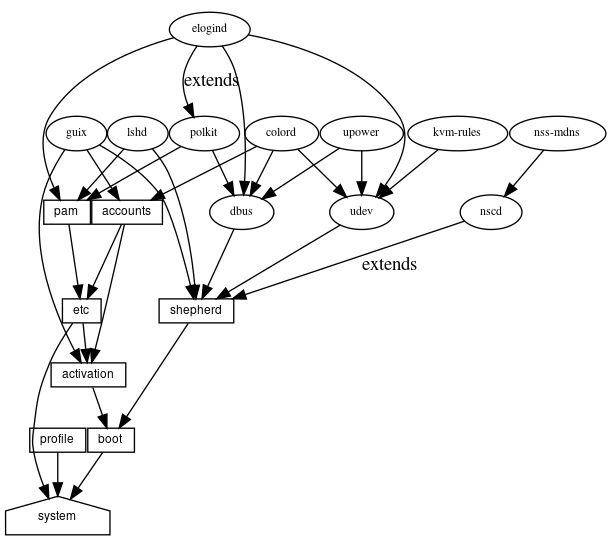
\includegraphics[width=0.75\columnwidth]{resources/service-graph.png}
  \end{center}
\end{frame}

\begin{frame}[fragile]{Service config}
  \begin{center}
    \begin{semiverbatim}
(define httpd-service-type
  (service-type
    (name 'httpd)
    (extensions
     (list (service-extension shepherd-root-service-type
                              httpd-shepherd-services)
           (service-extension activation-service-type
                              httpd-activation)
           (service-extension account-service-type
                              (const \%httpd-accounts))))
    (compose concatenate)
    (extend httpd-process-extensions)))
    \end{semiverbatim}
  \end{center}
\end{frame}

\begin{frame}[fragile]{Package definition}
  % Maybe highlight things
  % name & version
  % source
  \begin{semiverbatim}
(package
  (name "hello")
  (version "2.10")
  (source
    (origin (method url-fetch)
            (uri (string-append
                  "mirror://gnu/hello/hello-"
                  version ".tar.gz"))
            (sha256
             (base32
              "0ssi1wqq5fyh99vdlb9kzl7c9lng89ndq1i"))))
  (build-system gnu-build-system)
  (synopsis "Hello, GNU world: An example GNU package")
  (description "...")
  (home-page "https://www.gnu.org/software/hello/")
  (license gpl3+))
  \end{semiverbatim}
\end{frame}

% TODO: discuss the implications of `build-system` inside
% TODO: Add modify-phases
\begin{frame}[fragile]{Overriding packages}
  \begin{center}
    \begin{semiverbatim}
;; GnuTLS for Guile 2.0.
(package
  (inherit gnutls)
  (name "guile2.0-gnutls")
  (inputs `(("guile" ,guile-2.0)
            ,@(alist-delete "guile" (package-inputs gnutls))))))
    \end{semiverbatim}
  \end{center}
\end{frame}

\begin{frame}{Builders}
  \begin{multicols}{3}
    \begin{itemize}
      \item \textbf{gnu}
      \item ant
      \item android-ndk
      \item asdf
      \item cargo
      \item clojure
      \item cmake
      \item dune
      \item go
      \item glib
      \item guile
      \item minify
      \item ocaml
      \item python
      \item perl
      \item r
      \item rakudo
      \item texlive
      \item ruby
      \item waf
      \item scons
      \item haskell
      \item dub
      \item emacs
      \item \textbf{font}
      \item meson
      \item \textbf{linux-module}
      \item trivial
    \end{itemize}
  \end{multicols}
\end{frame}

\begin{frame}[fragile]{Third party packages - Go}
  \begin{center}
    \begin{semiverbatim}
(define go:\%standard-phases
  (modify-phases gnu:\%standard-phases
    (add-before 'unpack setup-go-environment)
    (replace 'unpack unpack)
    (delete 'bootstrap)
    (delete 'configure)
    (delete 'patch-generated-file-shebangs)
    (replace 'build build)
    (replace 'check check)
    (replace 'install install)
    (add-after 'install remove-go-references)))
    \end{semiverbatim}
  \end{center}
\end{frame}

\section{Is it any good?}

\begin{frame}{What I noticed while using}
  \begin{itemize}
    % Only examples, gui is better
    \item No `nixos-generate-config`
    % `/etc/shells` is built from all user's shells plus sh and bash
    % guix environment honors $SHELL
    \item Fish works flawlessly
    \item PS1 indicator for `guix environment`
    \item No `nixos-rebuild test`, only `switch`
    \item No /usr/bin/env by default, only /bin/sh
    % maintainer attribute but literally 6 uses, which are all bug-guix@gnu.org
    \item No package maintainers
    \item \%base-packages is small
  \end{itemize}
\end{frame}

% What would stop someone from using it
\begin{frame}{Limitations}
  \begin{itemize}
    % Would've put on my laptop next to NixOS otherwise
    % Should be easy, somebody tried 4 years ago
    % In NixOS looks like it's just: vgchange -ay
    \item No root FS on LVM
    \item Cannot build a package or run system test without compiling all guix modules
    \item Importing modules that have a syntax error doesn't give a helpful error
    % Doesn't have many proprietary drivers by default
    % And in general proprietary software is harder to get
    % Might be an advantage for you
    \item Linux-libre
  \end{itemize}
\end{frame}

\section{Compatibility}
\begin{frame}{Layers}
  \begin{itemize}
    \item Source
    \item (Bag)  % We don't have that
    \item Daemon
    % Incompatible because of different builtins
    % (looks like they just renamed builtins:fetchurl to builtins:download)
    \item Derivation
    \item Output % Compatible but useless to import into /nix/store because all paths would have to be rewritten
  \end{itemize}
\end{frame}

\section{Advantages \\What Nix can learn from Guix}

\begin{frame}{Advantages of Guix}
  \begin{itemize}
    \item Unique name: Way better to search for
      % TODO: Make this appear after
      \begin{itemize}
        \item Much less funny (if you're Dutch or German)
      \end{itemize}
    % Lots of configuration options, including encryption
    \item<+-> Graphical (ncurses) installer!
    \item<+-> Can combine `guix environment guix --ad-hoc git strace`!!
    \item<+-> Has `snippet` in addition to patches as a script to modify the sources
    % We don't but have last week decided against SELinux on NixOS
    \item<+-> Has SELinux policy (for foreign distros)
    \item<+-> Phases can be replaced while keeping "hooks"
    \item<+-> Native compilation for foreign archs with QEMU
    % Store contains only necessary closure!
    % Can even disable network
    \item<+-> `guix environment --container`
    \item<+-> `guix system container /etc/config.scm`
    \item<+-> Python3 is already default
  \end{itemize}
\end{frame}

\begin{frame}[fragile]{Grafts}
  Recursively rewrite all dependent packages
  \begin{center}
    \begin{semiverbatim}
(define bash
  (package
    (name "bash")
    ;; …
    (replacement bash-fixed)))
    \end{semiverbatim}
  \end{center}
\end{frame}

\begin{frame}{`guix pack`}
  \begin{itemize}
    \item<+-> Export runnable derivation as tarball %(docker or squashfs)
    \item<+-> But it has to write to `/gnu/store`
    \item<+-> Solution: Namespaces with `--relocatable`
  \end{itemize}
\end{frame}

\begin{frame}{What Nix can learn from Guix}
  \begin{itemize}
    \item Translation (Manual, synopses, description)
    \item Usability: More integrated and more opinionated
  \end{itemize}
\end{frame}

\begin{frame}{More integrated and opinionated}
  \begin{itemize}
    % Requires Emacs lol
    % Can even format just a single package in a file
    \item Official Code formatter
    % Eelco said yesterday, he's working on moving everything there
    \item Unified commandline, like Nix 2.0
    \item `guix deploy` is like NixOps % Haven't tried yet
    \item `guix lint`
    \item `guix import`
    \item `guix refresh` (Like r-ryantm)
  \end{itemize}
\end{frame}

\begin{frame}{guix lint}
  \begin{itemize}
    % Validate certain typographical and stylistic rules
    \item Synopsis, description
    \item inputs-should-be-native
    \item Check URLs, suggest mirror/GitHub
    % We've got this in nixpkgs-update
    \item CVE
    \item Formatting
  \end{itemize}
\end{frame}

\begin{frame}{guix import}
  Import from any of these package sets into Guix
  \begin{multicols}{2}
    \begin{itemize}
      \item gnu
      \item pypi
      \item gem
      \item cpan
      \item cran
      \item texlive
      \item json!
      \item nix % Doesn't work and throws lots of warnings
      \item hackage
      \item stackage
      \item elpa
      \item crate
      \item opam
    \end{itemize}
  \end{multicols}
\end{frame}

\begin{frame}{guix refresh}
  Update from any of these upstream sources

  \begin{multicols}{2}
    \begin{itemize}
      \item gnu
      \item gnome
      \item kde
      \item xorg
      \item kernel.org
      \item elpa
      \item cran
      \item bioconductor
      \item cpan
      \item pypi
      \item gem
      \item github
      \item hackage
      \item stackage
      \item launchpad
    \end{itemize}
  \end{multicols}
\end{frame}

\begin{frame}[fragile]{Nix' Channel Problems}
%Eelco's Talk: nix-channel
%  - not git repo
%  - can't easily pin a channel
%  - no inter-repo dependencies
  \begin{center}
    \begin{semiverbatim}
;; Tell 'guix pull' to use my own repo.
(list (channel
        (name 'guix)
        (url "https://example.org/my-guix.git")
        (branch "super-hacks")))

; Channel dependencies
(channel
 (version 0)
 (dependencies
  (channel
   (name some-collection)
   (url "https://example.org/evil/proprietary-pkgs.git"))))
    \end{semiverbatim}
  \end{center}
\end{frame}

\begin{frame}{Command comparison}
  \begin{tabular}{l|l}
    Nix & Guix \\
    \hline
    nixos-rebuild switch            & guix system reconfigure config.scm \\
    nixos-rebuild build             & guix system build config.cm        \\
    nixos-rebuild build-vm          & guix system vm config.scm          \\
    ---                             & guix system container config.scm   \\
    \hline
    nix-env -iA hello               & guix package -i hello              \\
    nix search foo                  & guix packages -s foo               \\
    nix-env -e hello                & guix packages -r hello             \\
    \hline
    nix-channel --update            & guix pull                          \\
    \hline
    nix-shell '<nixpkgs>' -A qemu   & guix environment qemu              \\
    nix-shell -p hello              & guix environment --ad-hoc hello    \\
    nix-shell default.nix           & guix environment -l default.scm    \\
    \hline
    nix-build '<nixpkgs>' hello     & guix build hello                   \\
    nix-build '<nixpkgs>' hello.src & guix build --source hello          \\
    nix-build default.nix           & guix build -f default.scm          \\
  \end{tabular}
\end{frame}

%\section{What can Nix users learn from Guix?}
%% You can use services to do everything
%% -> Don't rely on imports
%\section{Is it useful to install Guix?}
%\section{Can we synergize?}

\begin{frame}{Summary}
  \begin{itemize}
    \item Basically NixOS with Lisp instead of Nix\&Bash
    \item Service composition works differently % TODO: Better description
    \item More focus on free software
    \item Just like Nix: Small but dedicated community
    \item Nice and refreshing break from Nix (but not the ideas)
    \item Think of it like: Learn another language just to get better at your own
  \end{itemize}
\end{frame}

\appendix

\begin{frame}{Where development happens}
  \begin{center}
    \begin{tabular}{l|l|l}
      & Nix & Guix \\
      \hline
      Code          & GitHub Repo  & Savannah \\
      Contributing  & GitHub PR    & patches ML \\
      % Yes, they have a pretty web interface but it's just for viewing
      Issues        & GitHub Issue & bug ML \\
      Announcements & Discourse    & info ML \\
      Discussion    & Discourse    & devel ML \\
      Chat          & IRC          & IRC \\
    \end{tabular}
  \end{center}
\end{frame}

\begin{frame}{Sources of information}
  \begin{tabular}{l|l}
    % TODO: Make https:// grey
    Source            & https://git.savannah.gnu.org/cgit/guix.git \\
    Guile             & https://gnu.org/software/guile/manual \\
    Guix (\& OS)      & https://guix.gnu.org/manual \\
    Shepherd          & https://gnu.org/software/shepherd \\
    % Released last Tuesday
    \textbf{Cookbook} & https://guix.gnu.org/cookbook \\
    \textbf{Notes}    & https://gitlab.com/pjotrp/guix-notes \\
    Blog              & https://guix.gnu.org/blog \\
    Contributing      & https://guix.gnu.org/contribute \\
    \textbf{Videos}   & https://archive.org/details/guix-videos \\
    Reference Card    & https://guix.gnu.org/guix-refcard.pdf \\
    NEWS              & \\
    `guix --help`     & \\
    `info guix`       & \\
  \end{tabular}
\end{frame}

\begin{frame}{Comparison on numbers}
  \begin{center}
    \begin{tabular}{l|r|r}
      & Nix & Guix \\
      \hline
      % Last summer
      Packages       & 48.646    & 7.892 \\
      First commit   & 2003      & 2012 \\
      Commits        & 197.755   & 49.623 \\
      Contributors   & 3.624     & 330 \\
      % These numbers don't mean anything because we do things differently
      % or might have autogenerated files
      % NOTE: Took out everything except Nix&Scheme because, e.g. we've got 0.5m C??
      Nix/Guile SLOC & 1.257.944 & 465.692 \\  % tokei .
      Files          & 20.004    & 989
    \end{tabular}
  \end{center}
\end{frame}

\end{document}

% TODO
% - Downloads
%modify-services to change service
%config to instantiate service-type to service
%There's no .enable = false, you have to remove it from the list
%
%                   (remove (lambda (service)
%                             (eq? (service-kind service) gdm-service-type))
%                           %desktop-services))))
